\documentclass[a4paper,12pt]{scrartcl}
\usepackage[utf8]{inputenc}
\usepackage{amsmath}
\usepackage{bbold}

\usepackage{graphicx}
\usepackage{caption}
\usepackage{subcaption}
\usepackage[left=3cm,right=3cm,top=3.5cm,bottom=3.5cm]{geometry}
\usepackage{pgfplots,pgfplotstable}
\usepackage{tikz}
%\usetikzlibrary{positioning, fadings, through}
\usepackage{fancyhdr}
\usepackage[locale=DE,output-decimal-marker={.}]{siunitx}
\sisetup{separate-uncertainty, per-mode=fraction,}
\usepackage{here}
\usepackage{hyperref}

\usepackage{setspace}
\onehalfspacing
\usepackage{comment}

\usepackage{circledsteps}

% Default fixed font does not support bold face
\DeclareFixedFont{\ttb}{T1}{txtt}{bx}{n}{12} % for bold
\DeclareFixedFont{\ttm}{T1}{txtt}{m}{n}{12}  % for normal

% Custom colors
\usepackage{color}
\definecolor{deepblue}{rgb}{0,0,0.5}
\definecolor{deepred}{rgb}{0.6,0,0}
\definecolor{deepgreen}{rgb}{0,0.5,0}

\usepackage{listings}

% Python style for highlighting
\newcommand\pythonstyle{\lstset{
numbers=left,
language=Python,
basicstyle=\ttm,
otherkeywords={self},             % Add keywords here
% keywordstyle=\ttb\color{deepblue},
emph={MyClass,__init__},          % Custom highlighting
emphstyle=\ttb\color{deepred},    % Custom highlighting style
stringstyle=\color{deepgreen},
frame=tb,                         % Any extra options here
showstringspaces=false            % 
}}


% Python environment
\lstnewenvironment{python}[1][]{
\pythonstyle
\lstset{#1}
}{}

% Python for external files
\newcommand\pythonexternal[2][]{{
\pythonstyle
\lstinputlisting[#1]{#2}}}

% Python for inline
\newcommand\pythoninline[1]{{\pythonstyle\lstinline!#1!}}


\usepackage{booktabs}
\usepackage{multirow}
\usetikzlibrary{external}
\tikzexternalize[prefix=tikz/]

\pgfplotsset{compat=newest,
    tick label style={font=\small},
    label style={font=\small},
    legend style={font=\footnotesize}
    }
    
\tikzset{every mark/.append style={scale=0.3}}
\tikzset{>=stealth}
\usepackage{acronym}
\newlength{\plotheight}
\newlength{\plotwidth}
\newlength{\imgheight}
\setlength{\plotwidth}{14cm}
\setlength{\plotheight}{8cm}


\newcommand{\titel}{Fourier Modal Method}
\usepackage{fancyhdr}
\fancyhf{}
\pagestyle{fancy}
\cfoot{\thepage}
\fancyhead[L]{\leftmark}
\fancyhead[R]{\thepage}

\subject{Report}
\title{\titel}
\author{\large{Felix \textsc{Wechsler}, Tymoteusz \textsc{Wrzeszcz}, Joshua \textsc{Jordaan}}\\  \large{Group 2}}
\date{\large{\today}}
\publishers{\vspace{5.5cm}Abbe School of Photonics\\
            Friedrich-Schiller-Universität Jena}


\newcommand\todo[1]{\textcolor{red}{\textbf{TODO: #1}}}

%proper Integral typsetting
\newcommand{\dt}{\, \mathrm{d}t}
\newcommand{\dd}{\mathrm{d}}

\newcommand\ff[1]{ \mathbf #1(\mathbf r, \omega)}
\newcommand\lap{\mathop{{}\bigtriangleup}\nolimits}

\usepackage[%
  backend=biber,
  url=false,
  style=alphabetic,
  % citestyle=authoryear,
  maxnames=4,
  minnames=3,
  maxbibnames=99,
  giveninits,
uniquename=init]{biblatex}

\addbibresource{references.bib}
\pgfkeys{/csteps/inner color=transparent , /csteps/outer color=black}


%indentation to 0
\setlength\parindent{0pt}
\begin{document}
    \maketitle
	\thispagestyle{empty}
	\newpage
	\setcounter{page}{1}
	\tableofcontents

\newpage
\section{Introduction}
    In this report we show how to implement the Fourier Modal Method.
    In the first section we present the theoretical background of the method.
    Afterwards we give details on how to implement the numerical code.
    At the end we present some physical results of a diffraction grating and provide insights into speed 
    and numerical properties of the method.


\section{Physical Background}
    The general idea is to slice the grating into z-invariant layers. Then in each layer the Bloch periodic modes can be calculated. Since a grating structure is periodic, their definition also has to involve periodicity, and therefore they can be decomposed in Fourier basis. Therefore each eigenmode will have its Fourier coefficients which are nothing else but plane waves. The Next step is the propagation of calculated modes in single layer over distance equal to its thickness. At the interface between two layers, boundary conditions have to be fulfilled, i.e., transverse electric and magnetic fields have to be continuous across the interface. The Transfer matrix is then built from all layers, and connected to incident, and outgoing wave in homogeneous media. This way reflection and transmission problems can be easily solved. More detailed explanations of the algorithm are done below.\\
    
    
    The problem starts from the scalar wave equation for TE polarization, so $E_{y}(x)$ component has to determined. The wave propagates in $z$ direction, and has spatial dependence in $x$ direction. The ansatz for electric field amplitude reads as $E_{y}(x) = E_{y}exp(i\beta z)$, where $\beta$ is the propagation constant in $z$ direction. After plugging this ansatz in the wave equation we will get:
    
    \begin{equation}
        \frac{\partial^2 E_{y}(x)}{\partial x^2} + k_{0}^2\epsilon(x)E_{y}(x) = \beta^2E_{y}(x)
    \label{wave_eq}
    \end{equation}
    
    The next step is to apply Fourier expansion for both the electric field, and permittivity in each layer. Due to periodicity, the following condtions have to be fulfilled: $\epsilon(x + \Lambda)$ = $\epsilon(x)$, and $E_{y}(x + \Lambda) = exp(ik_{x}x)E_{y}(x)$, where $\Lambda$ is the period of the grating, and $k_{x}x$ is the quasi wavevector. Then the expansions will read as:
    
    \begin{align}
        \epsilon(x) &= \sum_{m=-\infty}^{\infty} \tilde{\epsilon}_{m}\exp(imGx)\\
        E_{y}(x) &= \sum_{m=-\infty}^{\infty} \tilde{\epsilon}_{m}\exp(i(k_{x} + mG)x)
    \label{expansions}
    \end{align}
    where $G = \frac{2\pi}{\Lambda}$ is the grating vector, and $\tilde\epsilon_{m}$ is the amplitude of the $m_{th}$ fourier component.\\
    After inserting these expansions in \autoref{wave_eq}, and converting to matrix notation one can obtain:
    
    \begin{equation}
        (k_{0}^2\boldsymbol{\hat{\epsilon}} - \boldsymbol{\hat{K}}^2) = \beta^2\boldsymbol{\phi}_{e}
    \label{mode_solver}
    \end{equation}
    
    where $\hat{K}$is a diagonal matrix which consists of $G_{m} + k_{x}$ entries, $\phi_{e}$ is the vector with Fourier coefficients that correspond to each mode, and $\hat{\epsilon}$ is the Toeplitz matrix which contains permittivity values.\\
    \autoref{mode_solver} is an eigenvalue problem which can be directly implemented and solved. The solution contains Fourier coefficients for all eigenmodes calcualted in a single layer.\\
    
    
    Fields are propagated in layers by multiplication with $\exp(\pm i\beta z)$, $+$ stands for forward progapating modes, and $-$ for backward propagating modes.
    In order to fulfill boundary conditions at the interface between two layers, the magnetic field $H_{x}$ has to be calculated. It can be computed simply from the curl equation for $H$, which results in $H_{x} = \beta E_{y}$. Boundary condition problem leads to the derivation of final form of layer transfer matrix. Amplitudes and phases of calculated modes are not known, and they are computed using this matrix. It reads as:
    
    \begin{align}
        \begin{split}
        \boldsymbol{\hat{T}} &=  \begin{bmatrix}
                                \boldsymbol{\hat{t}}_{11} & \boldsymbol{\hat{t}}_{12}\\
                                \boldsymbol{\hat{t}}_{21} & \boldsymbol{\hat{t}}_{22}
                                \end{bmatrix}  = \begin{bmatrix}
                                               \boldsymbol{I} & \boldsymbol{I}\\
                                               \hat{k_{z}}^{out} & -\hat{k_{z}}^{out}
                                               \end{bmatrix}^{-1}
                                               \displaystyle \\&
                                               \prod_{l} \left( \begin{bmatrix}
                                                                             \boldsymbol{\hat{\phi}}_{e}^l & \boldsymbol{\hat{\phi}}_{e}^l\\
                                                                             \boldsymbol{\hat{\phi}}_{e}^l\boldsymbol{\hat{\beta}}^l & -\boldsymbol{\hat{\phi}}_{e}^l\boldsymbol{\hat{\beta}}^l
                                                                             \end{bmatrix}  
                                                                             \begin{bmatrix}
                                                                                            \boldsymbol{\hat{p}}_{l}^{+} & 0\\
                                                                                            0 & \boldsymbol{\hat{p}}_{l}^{-}
                                                                                            \end{bmatrix}\begin{bmatrix}
                                                                                          \boldsymbol{\hat{\phi}}_{e}^l & \boldsymbol{\hat{\phi}}_{e}^l\\
                                                                                         \boldsymbol{\hat{\phi}}_{e}^l\boldsymbol{\hat{\beta}}^l &                     -\boldsymbol{\hat{\phi}}_{e}^l\boldsymbol{\hat{\beta}}^l
                                                                                             \end{bmatrix}^{-1}\right)        
                                                                                             \begin{bmatrix}
                                                                                                                    \boldsymbol{I} & \boldsymbol{I}\\
                                                                                                                    \hat{k_{z}}^{in} & -\hat{k_{z}}^{in}                                         \end{bmatrix} 
    \end{split}
    \label{transfer_m}   
    \end{align}
    where $\hat{k}_{z}^{out}$, $\hat{k}_{z}^{in}$ are propagation constants in the incoming, and outgoing media, and $\boldsymbol{\hat{p}}_{l}^{+}$, $\boldsymbol{\hat{p}}_{l}^{-}$ are propagators. Identity matrices show coefficients of the incoming and outgoing radiation, but since these media are homogeneous, modes are the plane waves which are defined by single 0th order Fourier coefficient.\\
    
    From the knowledge of system transfer matrix, reflected and transmitted complex amplitudes can be computed using:
    
    \begin{equation}
    \begin{split}
    \boldsymbol{r} = -\boldsymbol{\hat{t}}_{22}^{-1}\,\boldsymbol{\hat{t}}_{21}\,\boldsymbol{a}^{in}\\
    \boldsymbol{t} = (\boldsymbol{\hat{t}}_{11} - \boldsymbol{\hat{t}}_{12}\,\boldsymbol{\hat{t}}_{22}^{-1}\,\boldsymbol{\hat{t}}_{21})\,\boldsymbol{a}^{in}
    \end{split}
    \label{r_t}    
    \end{equation}
    
    which can be directly used to calculate diffraction efficiencies for reflection and transmission:
    
    \begin{equation}
    \begin{split}
    R_{m} = |r_{m}|^2\mathbf{Re}\left[\frac{\beta_{m}^{in}}{k_{z}^{in}}\right]\\
    T_{m} = |t_{m}|^2\mathbf{Re}\left[\frac{\beta_{m}^{out}}{k_{z}^{in}}\right]
    \label{efficiencies}    
    \end{split}
    \end{equation}
    
    It is worth to mention that the number of calculated diffraction orders can be checked easily since it can be also computed manually using Ewald construction.
    
    
 \section{Numerical Implementation}
    Implementation of the above mentioned algorithm is divided into two functions. First one \pythoninline{fmm1d_te_layer_modes} is responsible for calculation of TE eigenmodes in a single grating layer. Second one \pythoninline{fmm1d_te} computes diffraction efficiencies for a grating that consists of arbitrary number of layers.\\
    
    First function can be directly implemented using analytical equations, but there are some steps that have to be explained in more detail. One has to be careful about the output of \pythoninline{fft} function which sorts frequencies in some specific order, and only $2N$ negative and positive orders has to be picked up. It is also worth to mention that Toeplitz matrix defined with \pythoninline{toeplitz} function requires taking $0_{th}$ fourier coefficient twice for both negative and positive part. Eigenmodes are calculated as a set of fourier coefficients (eigenvectors) which create the structure of each mode. Eigenvalues are just propagation constants of each mode in a single layer. There is also one operation that has to be performed after solving the eigenvalue problem. Eigenvalues which correspond to backward propagating modes has to be inverted.\\
    
    Transfer matrix algorithm in the second function is a direct implementation of \autoref{transfer_m}. Structure of this matrix consists of block matrices with fourier coefficients for electric and magnetic field. There is also a block matrix with propagators that carry phase accumulated during propagation through each layer. This matrix product is calculated in a $for$ loop for each layer, and then multiplied with the previous result. To get the final transfer matrix, block matrices for incoming and outgoing material have to be specified. In the presented code it was done manually with analytical equations, but it could have been done using \pythoninline{fmm1d_te_layer_modes} function. After getting final form of transfer matrix, one can calculate reflection and transmission coefficients as well as efficiencies. They can be easily calculated using \autoref{expansions} and \autoref{mode_solver} by extracting different parts of transfer matrix. Most important aspect here is the definition of incoming field which is a plane wave. That is why all amplitudes of fourier coefficients are set to $0$ except the middle one which corresponds to $0_{th}$ order. It is also worth to mention that during calculation of diffraction efficiencies one has to ensure that right $\beta$ is chosen for the division. In the code it is denoted as \pythoninline{beta_in[N]} which is the propagation constant for $0_{th}$ order. For perpendicular incidence it will be equal to $k_{0}$ but as the incidence angle increases, $k_{x}$ component of wave vector is no longer $0$, and therefore this value will also change. So it is good to keep in mind that we are not dividing by a constant. 

    
    
    


% \newpage
\section{Results}
  
    
    \subsection{Computational Performance}
        In this section we provide some data for the computational performance.
        Our setup was Python 3.8.2, SciPy 1.3.2, NumPy 1.17.3 and a Intel(R) Core(TM) i7-7600U CPU @ 2.80GHz.
        The time needed for a 3 layer system and 20 positive Fourier order was \SI{0.0140\pm0.004}{\second} for single float precision.
        For double precision it was \SI{0.0134\pm0.002}{\second}. As it can be seen there is no significant difference. The computational demand of the numerical implementation is very low since most of the calculations are simple matrix multiplications or eigenvalue solutions of rather small matrices. Therefore, the limiting factor of the source code is Python as an interpreted language itself.
        
\subsection{Task 1: Layer modes}
The function \pythoninline{fmm1d_te_layer_modes} returns the effective propagation constants and the Fourier coefficients of the modes within the layer, up to the Fourier order considered. In order to extract the spatial field profiles an inverse Fourier transform was done on the mode Fourier coefficients. To do this the transformed mode had to be re-padded to the original permittivity vector size and arranged in the correct order that the inverse FFT was expecting. This was done using the test parameters provided in the Homework and the results of plotting the spatial profiles of propagating modes are shown below. Here the mode order shown refers to the Fourier order its associated $\beta_m$.
\begin{figure}[!h]
    \centering
    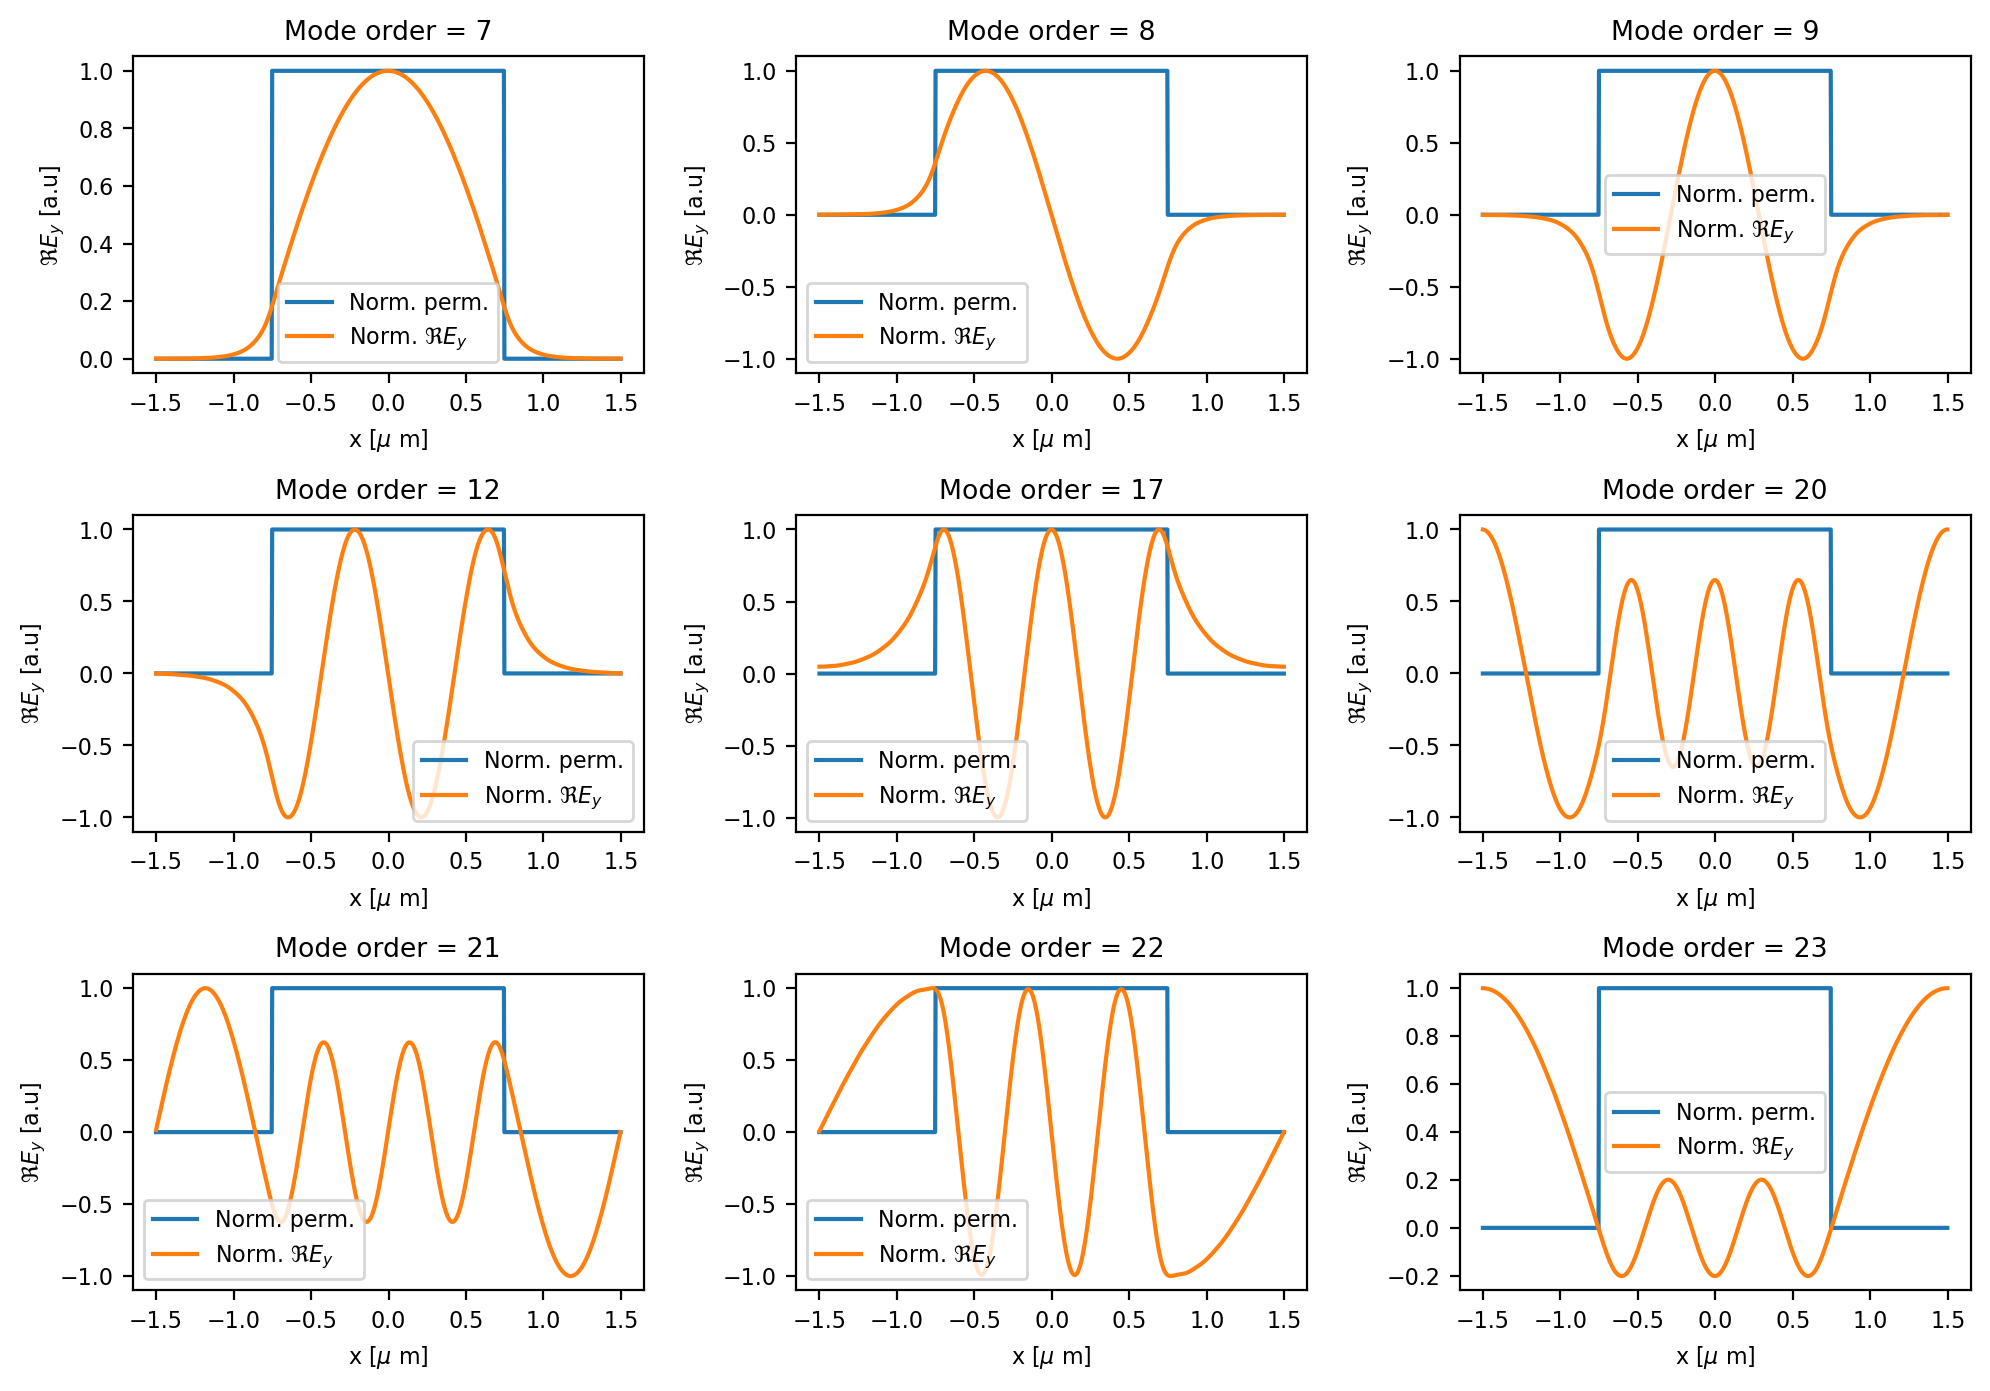
\includegraphics[width=0.99\textwidth]{figures/spatial_profile.png}
    \caption{Spatial profiles and effective refractive indices of the propagating modes.}
    \label{fig:saptial profiles}
\end{figure}
In Figure \ref{fig:saptial profiles} the symmetry of the permitivitty was shifted such that $x = 0$ coincides with the centre of the period, to make the profiles easier to interpret. The propagating modes were selected out all of the modes calculated for using the condition that the absolute value of the real part of $\beta_m$ is 10 orders of magnitude larger than the imaginary part. This condition was used rather than $\Im{\beta_m} = 0$, as all of the modes had some non-zero imaginary part of their propagation constant. 

From the results above we find that propagating modes are both guide and non-guided modes due to their spatial profile. We can also see that lower mode order corresponds to better guided modes, however how the mode order relates to this is more complex as there doesn't seem to be an immediately clear connection to the order spacing of propagating modes and when they begin.

\subsection{Task 2: Diffraction efficiencies of a multilayer grating}
From the output of \pythoninline{fmm1d_te} the transmitted and diffracted efficiencies can be immediately obtained without further processing. This was done for the test parameters described in the Homework sheet, and the results of the different angles of incidence are provided in Tables \ref{tab:eta t} and \ref{tab:eta r}. 
\begin{table}[!h]
\centering
\resizebox{\hsize}{!}{
\begin{tabular}{rrrrrrrrrrrrrrrrrrrrrr}
\toprule
 $\theta$ &  -10 &   -9 &   -8 &   -7 &   -6 &   -5 &   -4 &   -3 &   -2 &    -1 &    0 &    1 &    2 &     3 &    4 &    5 &    6 &    7 &    8 &    9 &   10 \\
\midrule
\SI{-30}{\degree} & 0.00 & 0.00 & 0.00 & 0.00 & 0.00 & 0.00 & 3.56 & 0.30 & 1.76 & 63.63 & 4.06 & 3.57 & 2.94 &  6.41 & 2.65 & 2.48 & 0.32 & 0.04 & 0.00 & 0.00 & 0.00 \\
  \SI{0}{\degree} & 0.00 & 0.00 & 0.00 & 0.00 & 0.00 & 1.82 & 6.78 & 0.99 & 0.10 & 53.50 & 3.61 & 3.11 & 2.47 & 10.73 & 4.76 & 4.96 & 0.00 & 0.00 & 0.00 & 0.00 & 0.00 \\
 \SI{30}{\degree} & 0.00 & 0.00 & 0.00 & 0.40 & 0.63 & 0.47 & 3.32 & 2.18 & 3.39 & 56.77 & 1.83 & 3.09 & 3.79 &  8.97 & 3.44 & 0.00 & 0.00 & 0.00 & 0.00 & 0.00 & 0.00 \\
\bottomrule
\end{tabular}}
    \caption{Transmitted diffraction efficiencies of the first 10 orders in units of percentage.}
    \label{tab:eta t}
\end{table}

\begin{table}[!h]
\centering
\resizebox{\hsize}{!}{
\begin{tabular}{rrrrrrrrrrrrrrrrrrrrrr}
\toprule
 $\theta$ &  -10 &   -9 &   -8 &   -7 &   -6 &   -5 &   -4 &   -3 &   -2 &   -1 &    0 &    1 &    2 &    3 &    4 &    5 &    6 &    7 &    8 &    9 &   10 \\
\midrule
\SI{-30}{\degree} & 0.00 & 0.00 & 0.00 & 0.00 & 0.00 & 0.00 & 0.00 & 0.00 & 0.00 & 0.87 & 0.82 & 2.86 & 3.65 & 0.01 & 0.05 & 0.00 & 0.00 & 0.00 & 0.00 & 0.00 & 0.00 \\
 \SI{0}{\degree} & 0.00 & 0.00 & 0.00 & 0.00 & 0.00 & 0.00 & 0.00 & 0.00 & 2.29 & 0.34 & 0.67 & 1.49 & 2.39 & 0.00 & 0.00 & 0.00 & 0.00 & 0.00 & 0.00 & 0.00 & 0.00 \\
 \SI{30}{\degree} & 0.00 & 0.00 & 0.00 & 0.00 & 0.00 & 0.00 & 1.05 & 3.39 & 1.83 & 0.47 & 0.82 & 4.15 & 0.00 & 0.00 & 0.00 & 0.00 & 0.00 & 0.00 & 0.00 & 0.00 & 0.00 \\
\bottomrule
\end{tabular}}
    \caption{Reflected diffraction efficiencies of the first 10 orders in units of percentage.}
    \label{tab:eta r}
\end{table}
From these results we find that the grating transmits mostly into the -1 order, with higher orders excited as the angle is changed from \SI{0}{\degree} incidence. This is as expected as the grating is transferring Bloch-momentum to the incident field and for off normal incidence this will add to the non-zero $k_x$ component. To better underdstand the behaviour of the grating it was also analysed for the whole range of angles \SI{89.99}{\degree} to \SI{-89.99}{\degree}. Exact values of \SI{90}{\degree} were avoided to exclude infinities in the solution. This is shown in the figures below.
\begin{figure}[!h]
    \centering
    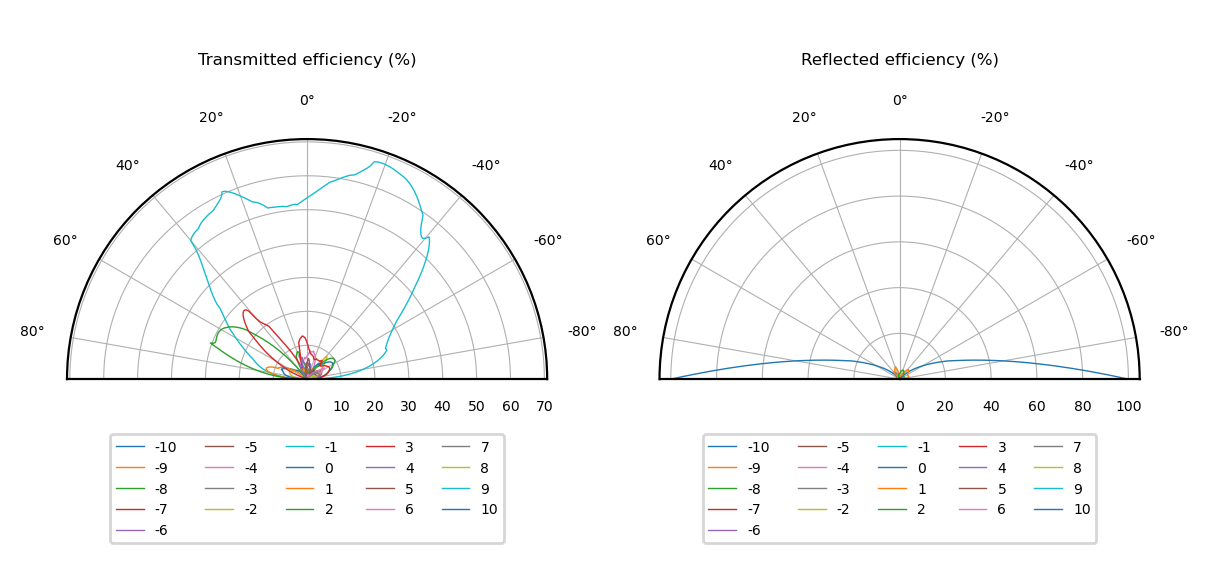
\includegraphics[width=\textwidth]{figures/efficiencies_plot.png}
    \caption{Diffracted efficiencies over full incident angle range.}
    \label{fig:effic plot}
\end{figure}

\begin{figure}[!h]
    \centering
    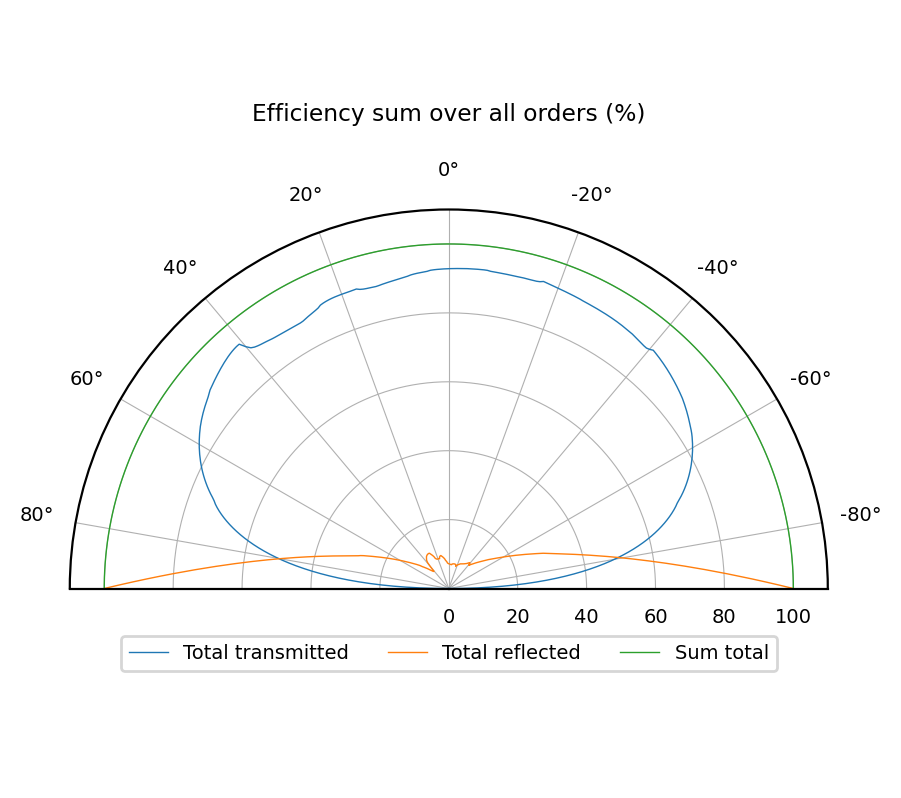
\includegraphics[width=0.5\textwidth]{figures/sum_efficiencies_plot.png}
    \caption{Sum over all orders of transmitted/reflected efficiencies and total sum.}
    \label{fig:sum effic plot}
\end{figure}
From Figure \ref{fig:effic plot} we can see that the dominant behaviour of the grating is overwhelmingly to transmit into the -1 order mode. We also find that transmission goes to 0 and reflection to 100\% at angles of $\pm\SI{90}{\degree}$, which is as expected. That the grating consistently transmits to the -1 diffraction order is due to its blazed grating profile where the order is preferenced by its blaze angle. The maximum transmission into this order occurs at around \SI{-19}{\degree}. From Figure \ref{fig:sum effic plot} we can also see that energy conservation is preserved in the simulation as all efficiencies sum to 100\% over the angular range. Figure \ref{fig:sum effic plot} again indicates how the grating operates primarily in transmission. 

\subsection{Side questions}
The side question parameters were also examined. It was found that in both cases; increasing the included diffraction orders to 40 or doubling the layer thickness, causes non-physical solutions to be outputted. This can be seen in Figure \ref{fig:effic sum side}, where the energy conservation condition in both cases are broken for all incidence angles. 
\begin{figure}
    \centering
    \begin{subfigure}[b]{0.46\textwidth}
        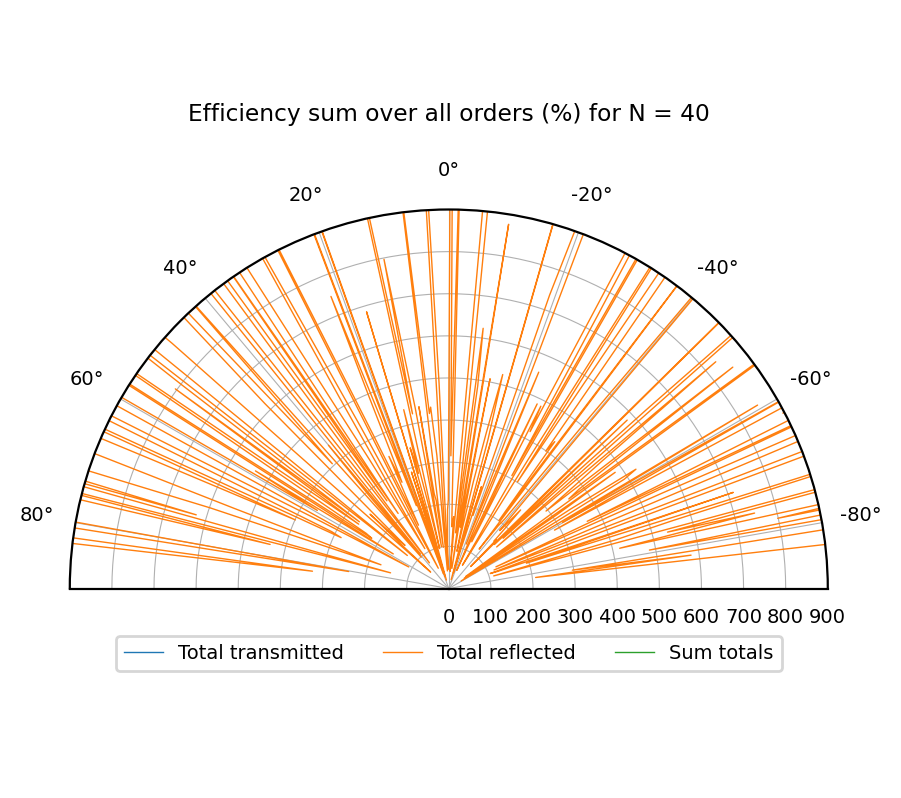
\includegraphics[width=\textwidth]{figures/sum_effic_N40.png}
    \end{subfigure}
    \begin{subfigure}[b]{0.46\textwidth}
        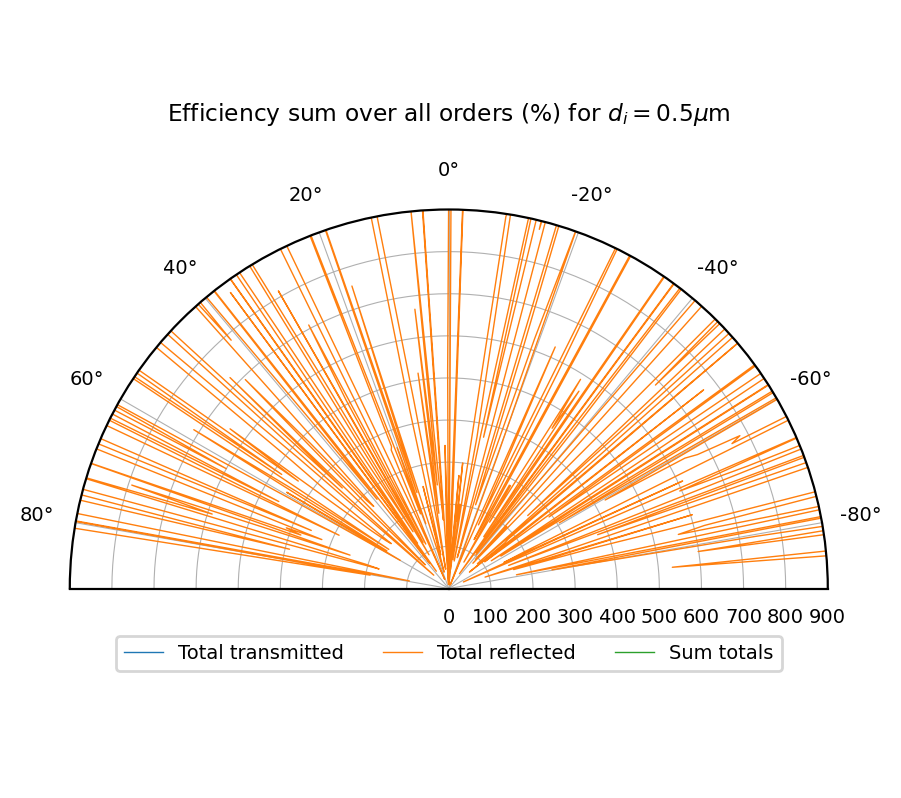
\includegraphics[width=\textwidth]{figures/sum_effic_d05.png}
    \end{subfigure}
    \caption{Efficiency sums for side question parameters.}
    \label{fig:effic sum side}
\end{figure}
These un-physical results are believed to be due to the instabilities of using the transfer matrix method in the algorithm, as discussed in the lectures. Specifically this is due to the phase propagation matrix and the $\boldsymbol{\hat{p}}_{l}^{\pm}$ terms. In the case of evanescent modes, as the phase is propagated both backwards and forwards, the results is in both a exponentially growing and shrinking term, which needs to be stored and solved in a single matrix and system of equations. For large values of $d_i$ this size of the length of the propagation increases such that the instabilities do as well, and similarly when including higher order Fourier components the prefactor in the exponential also increases which has the same affect as increasing $d_i$.

\section{Conclusion}
    In this report we presented details of the Fourier Modal method.
    We succeeded in applying this method on a blazed diffraction grating consisting of three different layers. We were able to extract the refraction and transmission efficiencies of the different orders.

\newpage
%to print all entries
\nocite{*}
\printbibliography


\end{document}